
\chapter{Testing \& Fazit}
\label{sec:testingfazit}
\todo{intro}

\section{Testing}
\label{sec:testingfazit:testing}
Nachfolgend werden die Richtigkeit des Programmes mit Hilfe der Testfälle aus \cref{sec:recherche:testcases} \nameref{sec:recherche:testcases} sowie der Hypothesen in \cref{sec:einleitung:ziel:hypothesen} \nameref{sec:einleitung:ziel:hypothesen} überprüft. Dabei werden die erwarteten Resultate mit den tatsächlichen Ausgaben des Programmes verglichen.

\subsection{Testfälle}
\label{sec:testingfazit:testing:testcases}
Dieser Abschnitt überprüft die Korrektheit der Algorithmen, also ob diese richtig Implementiert wurden. Dazu wurde im \cref{sec:recherche:testcases} Testfälle definiert inklusive der Einstellungen des Programmes.

Hier werden die Testfälle nochmals aufgeführt und mit den tatsächlichen Ausgaben des Proof of Concepts verglichen. Zum Ende jedes Tests ist das Ergebnis aufgeführt. \colorbox{green!25}{Grün} heisst das erwartete- stimmt mit dem tatsächlichen Resultat überein. Wenn dies nicht der Fall ist, dann ist das Ergebnis \colorbox{red!25}{rot}.

Alle Test sind erfolgreich. In \cref{fig:testingfazit:testing:testcases:uebersicht} wird eine Übersicht gegeben. In \cref{fig:testingfazit:testing:testcases:1} bis \cref{fig:testingfazit:testing:testcases:12:2} sind anschliessend alle Auswertung der Testfälle aufgeführt. Nach jeder Tabelle ist zusätzlich noch ein Bild vorhanden welches die Ausgabe des Programmes aufzeigt.

\begin{table}[H] 
	\caption{TC1 Auswertung}
	\centering
	%\rowcolors{1}{tablebodycolor}{tablerowcolor}
	\label{fig:testingfazit:testing:testcases:uebersicht}
	\begin{tabular}{ | l | l | l | l | l | } 
		\hline 
		\rowcolor{tableheadcolor}
		\bfseries ID & \bfseries Definition & \bfseries Auswertung & \bfseries Datenquelle & \bfseries Testergebniss\\ \hline 
		
		TC 1 & \cref{fig:recherche:testcases:1} & \cref{fig:testingfazit:testing:testcases:1} & \cref{app:testdatenquellen:1} & \cellcolor{green!25} \\ \hline 
		TC2 & \cref{fig:recherche:testcases:2} & \cref{fig:testingfazit:testing:testcases:2} & \cref{app:testdatenquellen:2} & \cellcolor{green!25} \\ \hline 
		TC3 & \cref{fig:recherche:testcases:3} & \cref{fig:testingfazit:testing:testcases:3} & \cref{app:testdatenquellen:3} & \cellcolor{green!25} \\ \hline 
		TC4 & \cref{fig:recherche:testcases:4} & \cref{fig:testingfazit:testing:testcases:4} & \cref{app:testdatenquellen:4} & \cellcolor{green!25} \\ \hline 
		TC5 & \cref{fig:recherche:testcases:5} & \cref{fig:testingfazit:testing:testcases:5} & \cref{app:testdatenquellen:5} & \cellcolor{green!25} \\ \hline 
		TC6 & \cref{fig:recherche:testcases:6} & \cref{fig:testingfazit:testing:testcases:6} & \cref{app:testdatenquellen:6} & \cellcolor{green!25} \\ \hline 
		TC7 & \cref{fig:recherche:testcases:7} & \cref{fig:testingfazit:testing:testcases:7} & \cref{app:testdatenquellen:7} & \cellcolor{green!25} \\ \hline 
		TC8 & \cref{fig:recherche:testcases:8} & \cref{fig:testingfazit:testing:testcases:8} & \cref{app:testdatenquellen:8} & \cellcolor{green!25} \\ \hline 
		TC9 & \cref{fig:recherche:testcases:9} & \cref{fig:testingfazit:testing:testcases:9} & \cref{app:testdatenquellen:9} & \cellcolor{green!25} \\ \hline 
		TC10 & \cref{fig:recherche:testcases:10} & \cref{fig:testingfazit:testing:testcases:10} & \cref{app:testdatenquellen:10} & \cellcolor{green!25} \\ \hline 
		TC11-1 & \cref{fig:recherche:testcases:11:1} & \cref{fig:testingfazit:testing:testcases:11:1} & \cref{app:testdatenquellen:11} & \cellcolor{green!25} \\ \hline 
		TC11-2 & \cref{fig:recherche:testcases:11:2} & \cref{fig:testingfazit:testing:testcases:11:2} & \cref{app:testdatenquellen:11} & \cellcolor{green!25} \\ \hline 
		TC12-1 & \cref{fig:recherche:testcases:12:1} & \cref{fig:testingfazit:testing:testcases:12:1} & \cref{app:testdatenquellen:12} & \cellcolor{green!25} \\ \hline 
		TC12-2 & \cref{fig:recherche:testcases:12:2} & \cref{fig:testingfazit:testing:testcases:12:2} & \cref{app:testdatenquellen:12} & \cellcolor{green!25} \\ \hline 
	\end{tabular}
\end{table}


\begin{table}[H] 
	\caption{TC1 Auswertung}
	\centering
	%\rowcolors{1}{tablebodycolor}{tablerowcolor}
	\label{fig:testingfazit:testing:testcases:1}
	\begin{tabular}{ | l | l | l | } 
		\hline 
		\rowcolor{tableheadcolor}
		\multicolumn{3}{|l|}{\bfseries ID: TC1} \\ \hline 
		Datebquelle & \multicolumn{2}{|l|}{\cref{app:testdatenquellen:1}} \\ \hline 
		Dateneinschränkung & \multicolumn{2}{|l|}{Keine} \\ \hline 
		
		\rowcolor{tableheadcolor}
		\multicolumn{3}{|l|}{\bfseries Erwartetes Resultat} \\ \hline 
		& Attributmenge & Anzahl \\ \hline 
		
		1er-Attributmenge & \tabitem Nahe am Wasser & 8 \\ \cline{2-3} 
		& \tabitem Nahe am Meer & 8 \\ \hline 
		
		2er-Attributmenge & \tabitem Nahe am Wasser & 8 \\
		& \tabitem Nahe am Meer & \\ \hline

		\rowcolor{tableheadcolor}
		\multicolumn{3}{|l|}{\bfseries Tatsächliches Resultat} \\ \hline 
		& Attributmenge & Anzahl \\ \hline 
		
		1er-Attributmenge & \tabitem Nahe am Wasser & 8 \\ \cline{2-3} 
		& \tabitem Nahe am Meer & 8 \\ \hline 
		
		2er-Attributmenge & \tabitem Nahe am Wasser & 8 \\
		& \tabitem Nahe am Meer & \\ \hline
		
		\rowcolor{tableheadcolor}
		\multicolumn{3}{|l|}{\bfseries Testergebnis} \\ \hline 
		\multicolumn{3}{|l|}{\cellcolor{green!25}} \\ \hline 
	\end{tabular}
\end{table}
\begin{figure}[H]
	\RawFloats
	\centering
	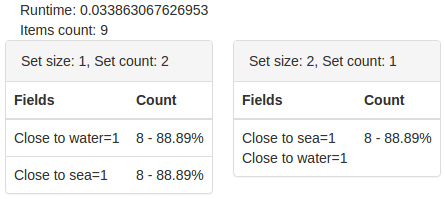
\includegraphics[width=0.5\textwidth]{images/tc1.png}
	\caption{TC1 - Ausgabe des Programmes}
	\label{fig:testingfazit:testing:testcases:1-1}
\end{figure}
\begin{table}[H] 
	\caption{TC2 Auswertung}
	\centering
	\label{fig:testingfazit:testing:testcases:2}
	\begin{tabular}{ | l | l | l | } 
		\hline 
		\rowcolor{tableheadcolor}
		\multicolumn{3}{|l|}{\bfseries ID: TC2} \\ \hline 
		Datebquelle & \multicolumn{2}{|l|}{\cref{app:testdatenquellen:2}} \\ \hline 
		Dateneinschränkung & \multicolumn{2}{|l|}{Keine} \\ \hline 
		
		\rowcolor{tableheadcolor}
		\multicolumn{3}{|l|}{\bfseries Erwartetes Resultat} \\ \hline 
		& Attributmenge & Anzahl \\ \hline 
		
		1er-Attributmenge & \tabitem Haustiere erlaubt & 8 \\ \cline{2-3} 
		& \tabitem Aircondition vorhanden & 8 \\ \hline 
		
		2er-Attributmenge & \tabitem Haustiere erlaubt & 8 \\
		& \tabitem Aircondition vorhanden & \\ \hline
		
		\rowcolor{tableheadcolor}
		\multicolumn{3}{|l|}{\bfseries Tatsächliches Resultat} \\ \hline 
		& Attributmenge & Anzahl \\ \hline 
		
		1er-Attributmenge & \tabitem Haustiere erlaubt & 8 \\ \cline{2-3} 
		& \tabitem Aircondition vorhanden & 8 \\ \hline 
		
		2er-Attributmenge & \tabitem Haustiere erlaubt & 8 \\
		& \tabitem Aircondition vorhanden & \\ \hline
		
		\rowcolor{tableheadcolor}
		\multicolumn{3}{|l|}{\bfseries Testergebnis} \\ \hline 
		\multicolumn{3}{|l|}{\cellcolor{green!25}} \\ \hline 
	\end{tabular}
\end{table}
\begin{figure}[H]
	\RawFloats
	\centering
	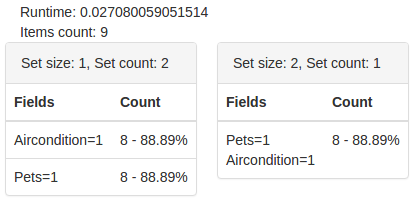
\includegraphics[width=0.5\textwidth]{images/tc2.png}
	\caption{TC2 - Ausgabe des Programmes}
	\label{fig:testingfazit:testing:testcases:2-1}
\end{figure}
\begin{table}[H] 
	\caption{TC3 Auswertung}
	\centering
	\label{fig:testingfazit:testing:testcases:3}
	\begin{tabular}{ | l | l | l | } 
		\hline 
		\rowcolor{tableheadcolor}
		\multicolumn{3}{|l|}{\bfseries ID: TC3} \\ \hline 
		Datebquelle & \multicolumn{2}{|l|}{\cref{app:testdatenquellen:3}} \\ \hline 
		Dateneinschränkung & \multicolumn{2}{|l|}{Keine} \\ \hline 
		
		\rowcolor{tableheadcolor}
		\multicolumn{3}{|l|}{\bfseries Erwartetes Resultat} \\ \hline 
		& Attributmenge & Anzahl \\ \hline 
		
		1er-Attributmenge & \tabitem Anzahl Zimmer=3 & 9 \\ \cline{2-3} 
		& \tabitem Anzahl Schlafzimmer=2 & 9 \\ \hline 
		
		2er-Attributmenge & \tabitem Anzahl Zimmer=3 & 9 \\
		& \tabitem Anzahl Schlafzimmer=2 & \\ \hline
		
		\rowcolor{tableheadcolor}
		\multicolumn{3}{|l|}{\bfseries Tatsächliches Resultat} \\ \hline 
		& Attributmenge & Anzahl \\ \hline 
		
		1er-Attributmenge & \tabitem Anzahl Zimmer=3 & 9 \\ \cline{2-3} 
		& \tabitem Anzahl Schlafzimmer=2 & 9 \\ \hline 
		
		2er-Attributmenge & \tabitem Anzahl Zimmer=3 & 9 \\
		& \tabitem Anzahl Schlafzimmer=2 & \\ \hline
		
		\rowcolor{tableheadcolor}
		\multicolumn{3}{|l|}{\bfseries Testergebnis} \\ \hline 
		\multicolumn{3}{|l|}{\cellcolor{green!25}} \\ \hline 
	\end{tabular}
\end{table}
\begin{figure}[H]
	\RawFloats
	\centering
	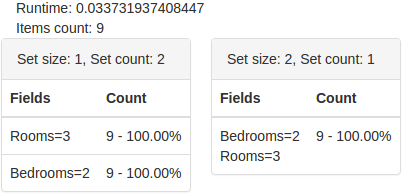
\includegraphics[width=0.5\textwidth]{images/tc3.png}
	\caption{TC3 - Ausgabe des Programmes}
	\label{fig:testingfazit:testing:testcases:3-1}
\end{figure}
\begin{table}[H] 
	\caption{TC4 Auswertung}
	\centering
	\label{fig:testingfazit:testing:testcases:4}
	\begin{tabular}{ | l | l | l | } 
		\hline 
		\rowcolor{tableheadcolor}
		\multicolumn{3}{|l|}{\bfseries ID: TC4} \\ \hline 
		Datebquelle & \multicolumn{2}{|l|}{\cref{app:testdatenquellen:4}} \\ \hline 
		Dateneinschränkung & \multicolumn{2}{|l|}{Keine} \\ \hline 
		
		\rowcolor{tableheadcolor}
		\multicolumn{3}{|l|}{\bfseries Erwartetes Resultat} \\ \hline 
		& Attributmenge & Anzahl \\ \hline 
		
		1er-Attributmenge & \tabitem Haustiere erlaubt & 8 \\ \cline{2-3} 
		& \tabitem Anzahl Schlafzimmer=3 & 9 \\ \hline 
		
		2er-Attributmenge & \tabitem Haustiere erlaubt & 8 \\
		& \tabitem Anzahl Schlafzimmer=3 & \\ \hline
		
		\rowcolor{tableheadcolor}
		\multicolumn{3}{|l|}{\bfseries Tatsächliches Resultat} \\ \hline 
		& Attributmenge & Anzahl \\ \hline 
		
		1er-Attributmenge & \tabitem Haustiere erlaubt & 8 \\ \cline{2-3} 
		& \tabitem Anzahl Schlafzimmer=3 & 9 \\ \hline 
		
		2er-Attributmenge & \tabitem Haustiere erlaubt & 8 \\
		& \tabitem Anzahl Schlafzimmer=3 & \\ \hline
		
		\rowcolor{tableheadcolor}
		\multicolumn{3}{|l|}{\bfseries Testergebnis} \\ \hline 
		\multicolumn{3}{|l|}{\cellcolor{green!25}} \\ \hline 
	\end{tabular}
\end{table}
\begin{figure}[H]
	\RawFloats
	\centering
	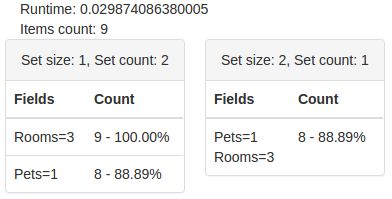
\includegraphics[width=0.5\textwidth]{images/tc4.png}
	\caption{TC4 - Ausgabe des Programmes}
	\label{fig:testingfazit:testing:testcases:4-1}
\end{figure}
\begin{table}[H] 
	\caption{TC5 Auswertung}
	\centering
	\label{fig:testingfazit:testing:testcases:5}
	\begin{tabular}{ | l | l | l | } 
		\hline 
		\rowcolor{tableheadcolor}
		\multicolumn{3}{|l|}{\bfseries ID: TC5} \\ \hline 
		Datebquelle & \multicolumn{2}{|l|}{\cref{app:testdatenquellen:5}} \\ \hline 
		Dateneinschränkung & \multicolumn{2}{|l|}{Haustiere erlaubt} \\ \hline 
		
		\rowcolor{tableheadcolor}
		\multicolumn{3}{|l|}{\bfseries Erwartetes Resultat} \\ \hline 
		& Attributmenge & Anzahl \\ \hline 
		
		1er-Attributmenge & \tabitem Nahe am Wasser & 4 \\ \cline{2-3} 
		& \tabitem Nahe am Meer & 5 \\ \hline 
		
		2er-Attributmenge & \tabitem Nahe am Wasser & 3 \\
		& \tabitem Nahe am Meer & \\ \hline
		
		\rowcolor{tableheadcolor}
		\multicolumn{3}{|l|}{\bfseries Tatsächliches Resultat} \\ \hline 
		& Attributmenge & Anzahl \\ \hline 
		
		1er-Attributmenge & \tabitem Nahe am Wasser & 4 \\ \cline{2-3} 
		& \tabitem Nahe am Meer & 5 \\ \hline 
		
		2er-Attributmenge & \tabitem Nahe am Wasser & 3 \\
		& \tabitem Nahe am Meer & \\ \hline
		
		\rowcolor{tableheadcolor}
		\multicolumn{3}{|l|}{\bfseries Testergebnis} \\ \hline 
		\multicolumn{3}{|l|}{\cellcolor{green!25}} \\ \hline 
	\end{tabular}
\end{table}
\begin{figure}[H]
	\RawFloats
	\centering
	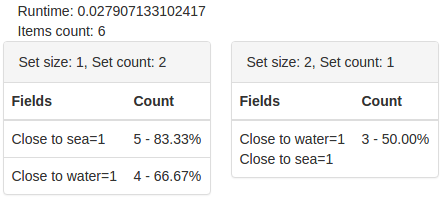
\includegraphics[width=0.5\textwidth]{images/tc5}
	\caption{TC5 - Ausgabe des Programmes}
	\label{fig:testingfazit:testing:testcases:5-1}
\end{figure}
\begin{table}[H] 
	\caption{TC6 Auswertung}
	\centering
	\label{fig:testingfazit:testing:testcases:6}
	\begin{tabular}{ | l | l | l | } 
		\hline 
		\rowcolor{tableheadcolor}
		\multicolumn{3}{|l|}{\bfseries ID: TC6} \\ \hline 
		Datebquelle & \multicolumn{2}{|l|}{\cref{app:testdatenquellen:6}} \\ \hline 
		Dateneinschränkung & \multicolumn{2}{|l|}{Nahe am ÖV (öffentlicher Verkehr)} \\ \hline 
		
		\rowcolor{tableheadcolor}
		\multicolumn{3}{|l|}{\bfseries Erwartetes Resultat} \\ \hline 
		& Attributmenge & Anzahl \\ \hline 
		
		1er-Attributmenge & \tabitem Nahe am Wasser & 3 \\ \cline{2-3} 
		& \tabitem Nahe am Meer & 4 \\ \hline 
		
		2er-Attributmenge & \tabitem Nahe am Wasser & 3 \\
		& \tabitem Nahe am Meer & \\ \hline
		
		\rowcolor{tableheadcolor}
		\multicolumn{3}{|l|}{\bfseries Tatsächliches Resultat} \\ \hline 
		& Attributmenge & Anzahl \\ \hline 
		
		1er-Attributmenge & \tabitem Nahe am Wasser & 3 \\ \cline{2-3} 
		& \tabitem Nahe am Meer & 4 \\ \hline 
		
		2er-Attributmenge & \tabitem Nahe am Wasser & 3 \\
		& \tabitem Nahe am Meer & \\ \hline
		
		\rowcolor{tableheadcolor}
		\multicolumn{3}{|l|}{\bfseries Testergebnis} \\ \hline 
		\multicolumn{3}{|l|}{\cellcolor{green!25}} \\ \hline 
	\end{tabular}
\end{table}
\begin{figure}[H]
	\RawFloats
	\centering
	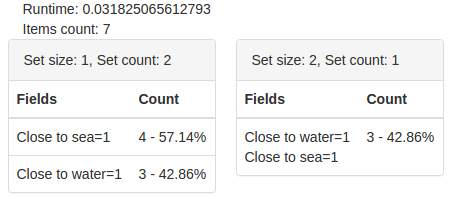
\includegraphics[width=0.5\textwidth]{images/tc6.png}
	\caption{TC6 - Ausgabe des Programmes}
	\label{fig:testingfazit:testing:testcases:6-1}
\end{figure}
\begin{table}[H] 
	\caption{TC7 Auswertung}
	\centering
	\label{fig:testingfazit:testing:testcases:7}
	\begin{tabular}{ | l | l | l | } 
		\hline 
		\rowcolor{tableheadcolor}
		\multicolumn{3}{|l|}{\bfseries ID: TC7} \\ \hline 
		Datebquelle & \multicolumn{2}{|l|}{\cref{app:testdatenquellen:7}} \\ \hline 
		Dateneinschränkung & \multicolumn{2}{|l|}{Anzahl Zimmer=3} \\ \hline 
		
		\rowcolor{tableheadcolor}
		\multicolumn{3}{|l|}{\bfseries Erwartetes Resultat} \\ \hline 
		& Attributmenge & Anzahl \\ \hline 
		
		1er-Attributmenge & \tabitem Nahe am Wasser & 6 \\ \cline{2-3} 
		& \tabitem Nahe am Meer & 4 \\ \hline 
		
		2er-Attributmenge & \tabitem Nahe am Wasser & 4 \\
		& \tabitem Nahe am Meer & \\ \hline
		
		\rowcolor{tableheadcolor}
		\multicolumn{3}{|l|}{\bfseries Tatsächliches Resultat} \\ \hline 
		& Attributmenge & Anzahl \\ \hline 
		
		1er-Attributmenge & \tabitem Nahe am Wasser & 6 \\ \cline{2-3} 
		& \tabitem Nahe am Meer & 4 \\ \hline 
		
		2er-Attributmenge & \tabitem Nahe am Wasser & 4 \\
		& \tabitem Nahe am Meer & \\ \hline
		
		\rowcolor{tableheadcolor}
		\multicolumn{3}{|l|}{\bfseries Testergebnis} \\ \hline 
		\multicolumn{3}{|l|}{\cellcolor{green!25}} \\ \hline 
	\end{tabular}
\end{table}
\begin{figure}[H]
	\RawFloats
	\centering
	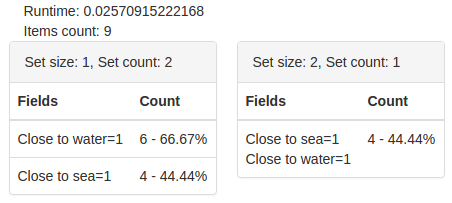
\includegraphics[width=0.5\textwidth]{images/tc7.png}
	\caption{TC7 - Ausgabe des Programmes}
	\label{fig:testingfazit:testing:testcases:7-1}
\end{figure}
\begin{table}[H] 
	\caption{TC8 Auswertung}
	\centering
	\label{fig:testingfazit:testing:testcases:8}
	\begin{tabular}{ | l | l | l | } 
		\hline 
		\rowcolor{tableheadcolor}
		\multicolumn{3}{|l|}{\bfseries ID: TC8} \\ \hline 
		Datebquelle & \multicolumn{2}{|l|}{\cref{app:testdatenquellen:8}} \\ \hline 
		Dateneinschränkung & \multicolumn{2}{|l|}{Keine} \\ \hline 
		
		\rowcolor{tableheadcolor}
		\multicolumn{3}{|l|}{\bfseries Erwartetes Resultat} \\ \hline 
		& Attributmenge & Anzahl \\ \hline 
		
		1er-Attributmenge & \tabitem Nahe am Wasser & 14 \\ \cline{2-3} 
		& \tabitem Nahe am Meer & 13 \\ \cline{2-3} 
		& \tabitem Haustiere erlaubt & 12 \\ \hline 
		
		2er-Attributmenge & \tabitem Nahe am Wasser & 11 \\
		& \tabitem Nahe am Meer & \\ \cline{2-3} 
		& \tabitem Nahe am Wasser & 10 \\
		& \tabitem Haustiere erlaubt & \\ \cline{2-3} 
		& \tabitem Nahe am Meer & 9 \\
		& \tabitem Haustiere erlaubt & \\ \hline
		
		3er-Attributmenge & \tabitem Nahe am Wasser & 8 \\
		& \tabitem Nahe am Meer & \\ 
		& \tabitem Haustiere erlaubt & \\ \hline
		
		\rowcolor{tableheadcolor}
		\multicolumn{3}{|l|}{\bfseries Tatsächliches Resultat} \\ \hline 
		& Attributmenge & Anzahl \\ \hline 
		
		1er-Attributmenge & \tabitem Nahe am Wasser & 14 \\ \cline{2-3} 
		& \tabitem Nahe am Meer & 13 \\ \cline{2-3} 
		& \tabitem Haustiere erlaubt & 12 \\ \hline 
		
		2er-Attributmenge & \tabitem Nahe am Wasser & 11 \\
		& \tabitem Nahe am Meer & \\ \cline{2-3} 
		& \tabitem Nahe am Wasser & 10 \\
		& \tabitem Haustiere erlaubt & \\ \cline{2-3} 
		& \tabitem Nahe am Meer & 9 \\
		& \tabitem Haustiere erlaubt & \\ \hline
		
		3er-Attributmenge & \tabitem Nahe am Wasser & 8 \\
		& \tabitem Nahe am Meer & \\ 
		& \tabitem Haustiere erlaubt & \\ \hline
		
		\rowcolor{tableheadcolor}
		\multicolumn{3}{|l|}{\bfseries Testergebnis} \\ \hline 
		\multicolumn{3}{|l|}{\cellcolor{green!25}} \\ \hline 
	\end{tabular}
\end{table}
\begin{figure}[H]
	\RawFloats
	\centering
	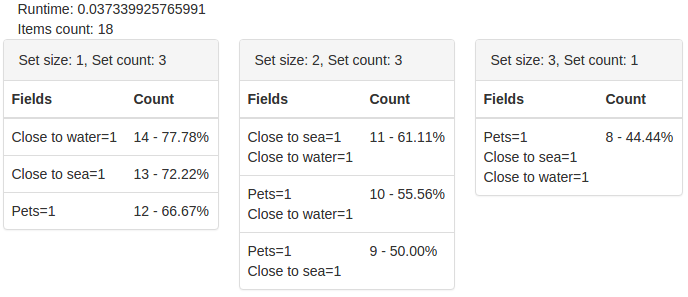
\includegraphics[width=1\textwidth]{images/tc8.png}
	\caption{TC8 - Ausgabe des Programmes}
	\label{fig:testingfazit:testing:testcases:8-1}
\end{figure}
\begin{table}[H] 
	\caption{TC9 Auswertung}
	\centering
	\label{fig:testingfazit:testing:testcases:9}
	\begin{tabular}{ | l | l | l | } 
		\hline 
		\rowcolor{tableheadcolor}
		\multicolumn{3}{|l|}{\bfseries ID: TC9} \\ \hline 
		Datebquelle & \multicolumn{2}{|l|}{\cref{app:testdatenquellen:9}} \\ \hline 
		Dateneinschränkung & \multicolumn{2}{|l|}{Keine} \\ \hline 
		
		\rowcolor{tableheadcolor}
		\multicolumn{3}{|l|}{\bfseries Erwartetes Resultat} \\ \hline 
		& Attributmenge & Anzahl \\ \hline 
		
		1er-Attributmenge & \tabitem Nahe am Wasser & 8 \\ \cline{2-3} 
		& \tabitem Nahe am Meer & 8 \\ \cline{2-3} 
		& \tabitem Haustiere erlaubt & 9 \\ \cline{2-3} 
		& \tabitem Anzahl Zimmer=3 & 11 \\ \hline
		
		2er-Attributmenge & \tabitem Nahe am Wasser & 8 \\
		& \tabitem Nahe am Meer & \\ \cline{2-3} 
		& \tabitem Haustiere erlaubt & 9 \\
		& \tabitem Anzahl Zimmer=3 & \\ \hline
		
		\rowcolor{tableheadcolor}
		\multicolumn{3}{|l|}{\bfseries Tatsächliches Resultat} \\ \hline 
		& Attributmenge & Anzahl \\ \hline 
		
		1er-Attributmenge & \tabitem Nahe am Wasser & 8 \\ \cline{2-3} 
		& \tabitem Nahe am Meer & 8 \\ \cline{2-3} 
		& \tabitem Haustiere erlaubt & 9 \\ \cline{2-3} 
		& \tabitem Anzahl Zimmer=3 & 11 \\ \hline
		
		2er-Attributmenge & \tabitem Nahe am Wasser & 8 \\
		& \tabitem Nahe am Meer & \\ \cline{2-3} 
		& \tabitem Haustiere erlaubt & 9 \\
		& \tabitem Anzahl Zimmer=3 & \\ \hline
		
		\rowcolor{tableheadcolor}
		\multicolumn{3}{|l|}{\bfseries Testergebnis} \\ \hline 
		\multicolumn{3}{|l|}{\cellcolor{green!25}} \\ \hline 
	\end{tabular}
\end{table}
\begin{figure}[H]
	\RawFloats
	\centering
	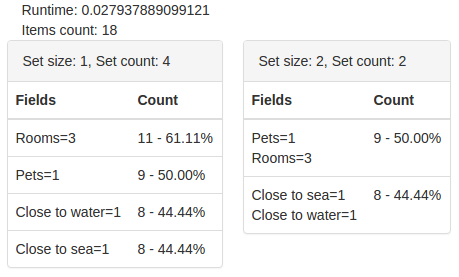
\includegraphics[width=0.5\textwidth]{images/tc9.png}
	\caption{TC9 - Ausgabe des Programmes}
	\label{fig:testingfazit:testing:testcases:9-1}
\end{figure}
\begin{longtable}{ | l | l | l | l |} 	
	\hline 
	\rowcolor{tableheadcolor}
	\multicolumn{4}{|l|}{\bfseries ID: TC10} \\ \hline 
	Datebquelle & \multicolumn{3}{|l|}{\cref{app:testdatenquellen:10}} \\ \hline 
	Dateneinschränkung & \multicolumn{3}{|l|}{Keine} \\ \hline 
	
	\rowcolor{tableheadcolor}
	\multicolumn{4}{|l|}{\bfseries Erwartetes Resultat} \\ \hline 
	Noise Punkte & \multicolumn{3}{|l|}{0} \\ \hline 
	
	% ----------------------------------------------		
	\multicolumn{4}{|l|}{\textbf{Cluster 1}} \\ \cline{2-4} 
	& Fehler & \multicolumn{2}{|l|}{0} \\ \cline{2-4} 
	& Grösse & \multicolumn{2}{|l|}{5} \\ \cline{2-4} 
	&& Attributmenge & Anzahl \\ \cline{2-4} 
	
	& 1er-Attributmenge & \tabitem Nahe am Wasser & 5 \\ \cline{3-4} 
	& & \tabitem Nahe am Meer & 5 \\ \cline{3-4} 
	& & \tabitem Anzahl Zimmer=3 & 5 \\ \cline{3-4} 
	& & \tabitem Anzahl Schlafzimmer=2 & 5 \\ \cline{2-4} 
	
	& 2er-Attributmenge & \tabitem Nahe am Wasser & 5 \\
	& & \tabitem Nahe am Meer & \\ \cline{3-4} 
	& & \tabitem Nahe am Wasser & 5 \\
	& & \tabitem Anzahl Zimmer=3 & \\ \cline{3-4} 
	& & \tabitem Nahe am Wasser & 5 \\
	& & \tabitem Anzahl Schlafzimmer=2 & \\ \cline{3-4} 
	
	& & \tabitem Nahe am Meer & 5 \\
	& & \tabitem Anzahl Zimmer=3 & \\ \cline{3-4} 
	& & \tabitem Nahe am Meer & 5 \\
	& & \tabitem Anzahl Schlafzimmer=2 & \\ \cline{3-4} 
	
	& & \tabitem Anzahl Zimmer=3 & 5 \\
	& & \tabitem Anzahl Schlafzimmer=2 & \\ \cline{2-4} 
	
	& 3er-Attributmenge & \tabitem Nahe am Wasser & 5 \\
	& & \tabitem Nahe am Meer & \\ 
	& & \tabitem Anzahl Zimmer=3 & \\ \cline{3-4} 
	& & \tabitem Nahe am Wasser & 5 \\
	& & \tabitem Nahe am Meer & \\ 
	& & \tabitem Anzahl Schlafzimmer=2 & \\ \cline{3-4}
	& & \tabitem Nahe am Meer & 5 \\
	& & \tabitem Anzahl Zimmer=3 & \\ 
	& & \tabitem Anzahl Schlafzimmer=2 & \\ \cline{3-4}
	& & \tabitem Nahe am Wasser & 5 \\
	& & \tabitem Anzahl Zimmer=3 & \\ 
	& & \tabitem Anzahl Schlafzimmer=2 & \\ \cline{2-4}
	
	& 4er-Attributmenge & \tabitem Nahe am Wasser & 5 \\
	& & \tabitem Nahe am Meer & \\ 
	& & \tabitem Anzahl Zimmer=3 & \\ 
	& & \tabitem Anzahl Schlafzimmer=2 & \\ \hline
	
	% ----------------------------------------------
	\multicolumn{4}{|l|}{\textbf{Cluster 2}} \\ \cline{2-4} 
	& Fehler & \multicolumn{2}{|l|}{0} \\ \cline{2-4} 
	& Grösse & \multicolumn{2}{|l|}{4} \\ \cline{2-4} 
	& & Attributmenge & Anzahl \\ \cline{2-4} 
	
	& 1er-Attributmenge & \tabitem Wochenpreis=günstig & 4 \\ \cline{3-4}
	& & \tabitem Anzahl Zimmer=9 & 4 \\ \cline{3-4}
	& & \tabitem Anzahl Schlafzimmer=9 & 4 \\ \cline{2-4} 
	
	& 2er-Attributmenge & \tabitem Wochenpreis=günstig & 4 \\
	& & \tabitem Anzahl Zimmer=9 & \\ \cline{3-4}
	& & \tabitem Wochenpreis=günstig & 4 \\
	& & \tabitem Anzahl Schlafzimmer=9 & \\ \cline{3-4} 
	& & \tabitem Anzahl Zimmer=9 & 4 \\
	& & \tabitem Anzahl Schlafzimmer=9 & \\ \cline{2-4}
	
	& 3er-Attributmenge & \tabitem Wochenpreis=günstig & 4 \\
	& & \tabitem Anzahl Zimmer=9 & \\ 
	& & \tabitem Anzahl Schlafzimmer=9 & \\ \hline
	
	\rowcolor{tableheadcolor}
	\multicolumn{4}{|l|}{\bfseries Tatsächliches Resultat} \\ \hline 
	Noise Punkte & \multicolumn{3}{|l|}{0} \\ \hline 
	
	% ----------------------------------------------		
	\multicolumn{4}{|l|}{\textbf{Cluster 1}} \\ \cline{2-4} 
	& Fehler & \multicolumn{2}{|l|}{0} \\ \cline{2-4} 
	& Grösse & \multicolumn{2}{|l|}{5} \\ \cline{2-4} 
	&& Attributmenge & Anzahl \\ \cline{2-4} 
	
	& 1er-Attributmenge & \tabitem Nahe am Wasser & 5 \\ \cline{3-4} 
	& & \tabitem Nahe am Meer & 5 \\ \cline{3-4} 
	& & \tabitem Anzahl Zimmer=3 & 5 \\ \cline{3-4} 
	& & \tabitem Anzahl Schlafzimmer=2 & 5 \\ \cline{2-4} 
	
	& 2er-Attributmenge & \tabitem Nahe am Wasser & 5 \\
	& & \tabitem Nahe am Meer & \\ \cline{3-4} 
	& & \tabitem Nahe am Wasser & 5 \\
	& & \tabitem Anzahl Zimmer=3 & \\ \cline{3-4} 
	& & \tabitem Nahe am Wasser & 5 \\
	& & \tabitem Anzahl Schlafzimmer=2 & \\ \cline{3-4} 
	
	& & \tabitem Nahe am Meer & 5 \\
	& & \tabitem Anzahl Zimmer=3 & \\ \cline{3-4} 
	& & \tabitem Nahe am Meer & 5 \\
	& & \tabitem Anzahl Schlafzimmer=2 & \\ \cline{3-4} 
	
	& & \tabitem Anzahl Zimmer=3 & 5 \\
	& & \tabitem Anzahl Schlafzimmer=2 & \\ \cline{2-4} 
	
	& 3er-Attributmenge & \tabitem Nahe am Wasser & 5 \\
	& & \tabitem Nahe am Meer & \\ 
	& & \tabitem Anzahl Zimmer=3 & \\ \cline{3-4} 
	& & \tabitem Nahe am Wasser & 5 \\
	& & \tabitem Nahe am Meer & \\ 
	& & \tabitem Anzahl Schlafzimmer=2 & \\ \cline{3-4}
	& & \tabitem Nahe am Meer & 5 \\
	& & \tabitem Anzahl Zimmer=3 & \\ 
	& & \tabitem Anzahl Schlafzimmer=2 & \\ \cline{3-4}
	& & \tabitem Nahe am Wasser & 5 \\
	& & \tabitem Anzahl Zimmer=3 & \\ 
	& & \tabitem Anzahl Schlafzimmer=2 & \\ \cline{2-4}
	
	& 4er-Attributmenge & \tabitem Nahe am Wasser & 5 \\
	& & \tabitem Nahe am Meer & \\ 
	& & \tabitem Anzahl Zimmer=3 & \\ 
	& & \tabitem Anzahl Schlafzimmer=2 & \\ \hline
	
	% ----------------------------------------------
	\multicolumn{4}{|l|}{\textbf{Cluster 2}} \\ \cline{2-4} 
	& Fehler & \multicolumn{2}{|l|}{0} \\ \cline{2-4} 
	& Grösse & \multicolumn{2}{|l|}{4} \\ \cline{2-4} 
	& & Attributmenge & Anzahl \\ \cline{2-4} 
	
	& 1er-Attributmenge & \tabitem Wochenpreis=günstig & 4 \\ \cline{3-4}
	& & \tabitem Anzahl Zimmer=9 & 4 \\ \cline{3-4}
	& & \tabitem Anzahl Schlafzimmer=9 & 4 \\ \cline{2-4} 
	
	& 2er-Attributmenge & \tabitem Wochenpreis=günstig & 4 \\
	& & \tabitem Anzahl Zimmer=9 & \\ \cline{3-4}
	& & \tabitem Wochenpreis=günstig & 4 \\
	& & \tabitem Anzahl Schlafzimmer=9 & \\ \cline{3-4} 
	& & \tabitem Anzahl Zimmer=9 & 4 \\
	& & \tabitem Anzahl Schlafzimmer=9 & \\ \cline{2-4}
	
	& 3er-Attributmenge & \tabitem Wochenpreis=günstig & 4 \\
	& & \tabitem Anzahl Zimmer=9 & \\ 
	& & \tabitem Anzahl Schlafzimmer=9 & \\ \hline
	
	\rowcolor{tableheadcolor}
	\multicolumn{4}{|l|}{\bfseries Testergebnis} \\ \hline 
	\multicolumn{4}{|l|}{\cellcolor{green!25}} \\ \hline 
	
	\caption{TC10 Auswertung}
	\centering
	\label{fig:testingfazit:testing:testcases:10}
\end{longtable}
\begin{figure}[H]
	\begin{subfigure}[t]{1\textwidth}
		\centering
		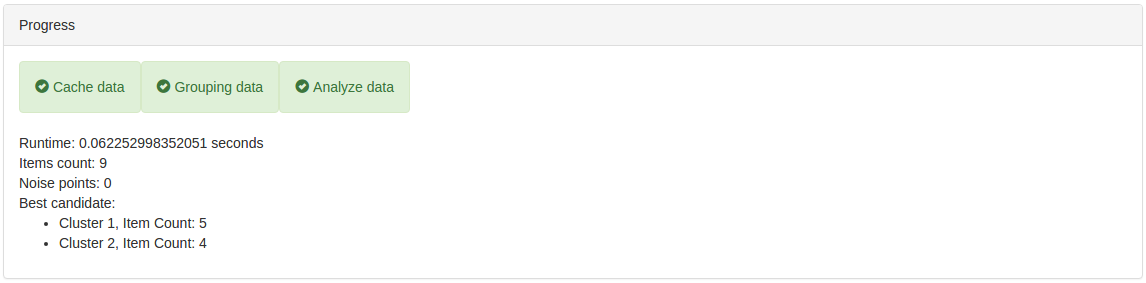
\includegraphics[width=1\textwidth]{images/tc10-dbscan-1}
		\caption{Generelle Informationen}
		\label{fig:testingfazit:testing:testcases:10-1-1}
	\end{subfigure} \\
	\begin{subfigure}[t]{1\textwidth}
		\centering
		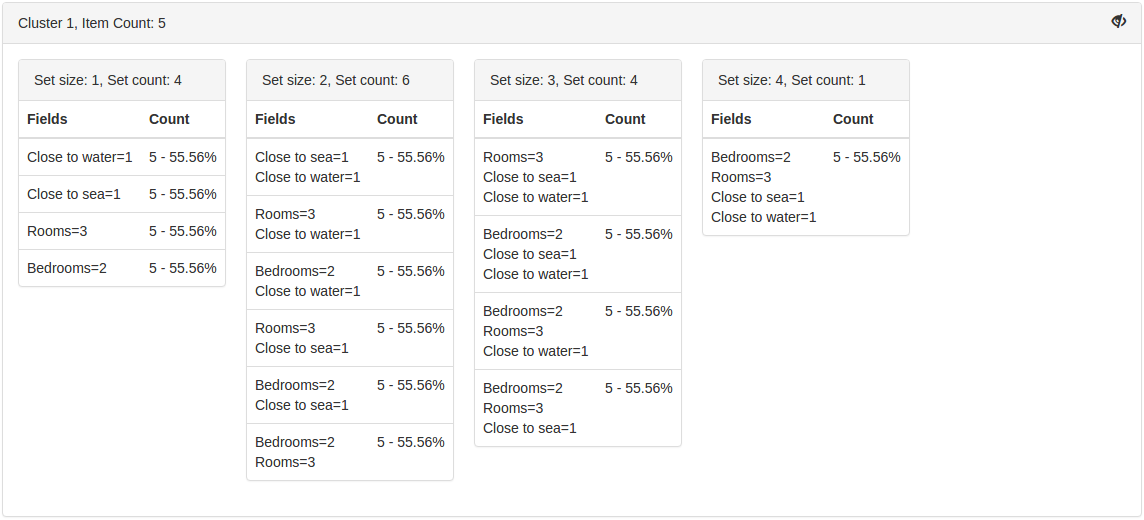
\includegraphics[width=1\textwidth]{images/tc10-dbscan-2}
		\caption{Cluster 1}
		\label{fig:testingfazit:testing:testcases:10-1-2}
	\end{subfigure}
	\begin{subfigure}[t]{1\textwidth}
		\centering
		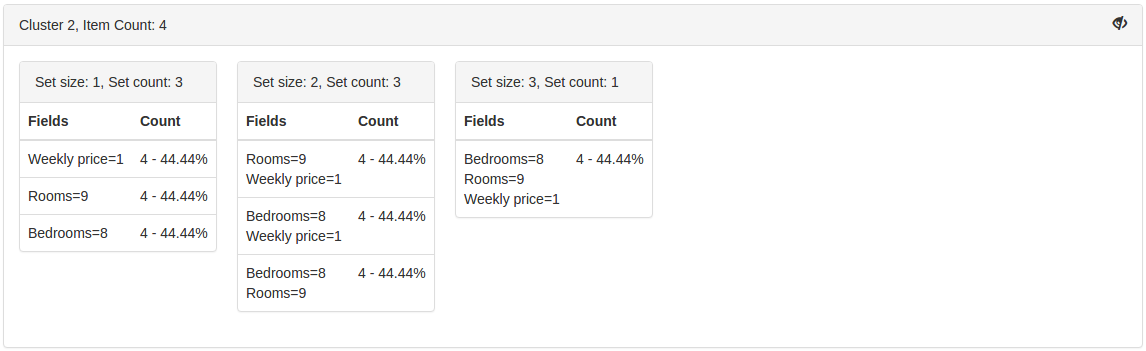
\includegraphics[width=1\textwidth]{images/tc10-dbscan-3}
		\caption{Cluster 2}
		\label{fig:testingfazit:testing:testcases:10-1-3}
	\end{subfigure}
	\caption{TC10 - Ausgabe des Programmes - Resultat des DBSCAN Algorithmus}
	\label{fig:testingfazit:testing:testcases:10-1}
\end{figure}
\begin{figure}[H]
	\begin{subfigure}[t]{1\textwidth}
		\centering
		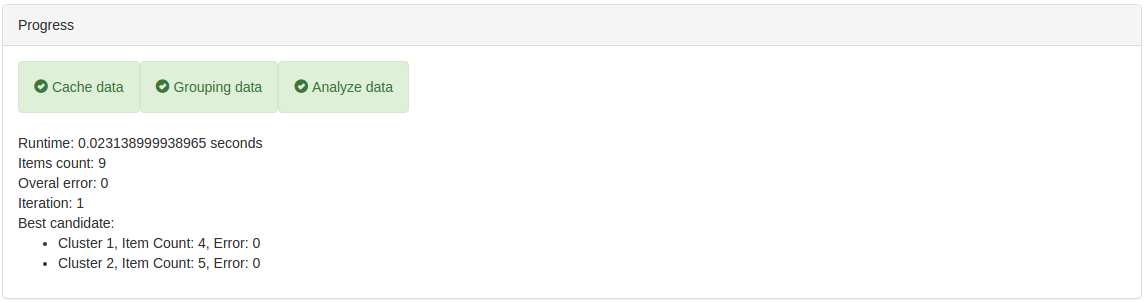
\includegraphics[width=1\textwidth]{images/tc10-kprototype-1}
		\caption{Generelle Informationen}
		\label{fig:testingfazit:testing:testcases:10-2-1}
	\end{subfigure} \\
	\begin{subfigure}[t]{1\textwidth}
		\centering
		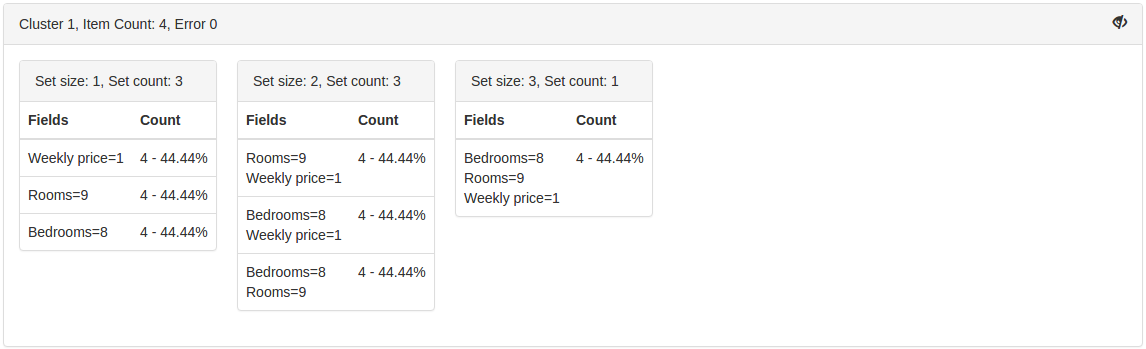
\includegraphics[width=1\textwidth]{images/tc10-kprototype-2}
		\caption{Cluster 1}
		\label{fig:testingfazit:testing:testcases:10-2-2}
	\end{subfigure}
	\begin{subfigure}[t]{1\textwidth}
		\centering
		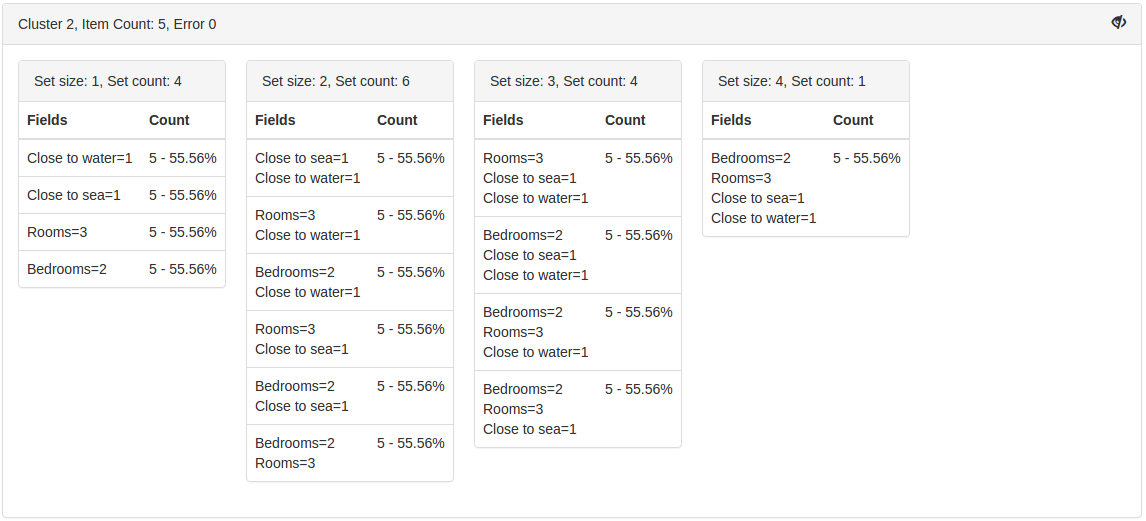
\includegraphics[width=1\textwidth]{images/tc10-kprototype-3}
		\caption{Cluster 2}
		\label{fig:testingfazit:testing:testcases:10-2-3}
	\end{subfigure}
	\caption{TC10 - Ausgabe des Programmes - Resultat des k-prototype Algorithmus}
	\label{fig:testingfazit:testing:testcases:10-2}
\end{figure}
\begin{longtable}{ | l | l | l | l |} 	
	\hline 
	\rowcolor{tableheadcolor}
	\multicolumn{4}{|l|}{\bfseries ID: TC11-1 DBSCAN} \\ \hline 
	Datebquelle & \multicolumn{3}{|l|}{\cref{app:testdatenquellen:11}} \\ \hline 
	Dateneinschränkung & \multicolumn{3}{|l|}{Keine} \\ \hline 
	
	\rowcolor{tableheadcolor}
	\multicolumn{4}{|l|}{\bfseries Erwartetes Resultat} \\ \hline 
	Noise Punkte & \multicolumn{3}{|l|}{1} \\ \hline 
	
	% ----------------------------------------------		
	\multicolumn{4}{|l|}{\textbf{Cluster 1}} \\ \cline{2-4} 
	& Grösse & \multicolumn{2}{|l|}{9} \\ \cline{2-4} 
	&& Attributmenge & Anzahl \\ \cline{2-4} 
	
	& 1er-Attributmenge & \tabitem Nahe am Wasser & 9 \\ \cline{3-4} 
	& & \tabitem Nahe am Meer & 9 \\ \cline{3-4} 
	& & \tabitem Anzahl Zimmer=3 & 9 \\ \cline{3-4} 
	& & \tabitem Anzahl Schlafzimmer=2 & 9 \\ \cline{2-4} 
	
	& 2er-Attributmenge & \tabitem Nahe am Wasser & 9 \\
	& & \tabitem Nahe am Meer & \\ \cline{3-4} 
	& & \tabitem Nahe am Wasser & 9 \\
	& & \tabitem Anzahl Zimmer=3 & \\ \cline{3-4} 
	& & \tabitem Nahe am Wasser & 9 \\
	& & \tabitem Anzahl Schlafzimmer=2 & \\ \cline{3-4} 
	
	& & \tabitem Nahe am Meer & 9 \\
	& & \tabitem Anzahl Zimmer=3 & \\ \cline{3-4} 
	& & \tabitem Nahe am Meer & 9 \\
	& & \tabitem Anzahl Schlafzimmer=2 & \\ \cline{3-4} 
	
	& & \tabitem Anzahl Zimmer=3 & 9 \\
	& & \tabitem Anzahl Schlafzimmer=2 & \\ \cline{2-4} 
	
	& 3er-Attributmenge & \tabitem Nahe am Wasser & 9 \\
	& & \tabitem Nahe am Meer & \\ 
	& & \tabitem Anzahl Zimmer=3 & \\ \cline{3-4} 
	& & \tabitem Nahe am Wasser & 9 \\
	& & \tabitem Nahe am Meer & \\ 
	& & \tabitem Anzahl Schlafzimmer=2 & \\ \cline{3-4}
	& & \tabitem Nahe am Meer & 9 \\
	& & \tabitem Anzahl Zimmer=3 & \\ 
	& & \tabitem Anzahl Schlafzimmer=2 & \\ \cline{3-4}
	& & \tabitem Nahe am Wasser & 9 \\
	& & \tabitem Anzahl Zimmer=3 & \\ 
	& & \tabitem Anzahl Schlafzimmer=2 & \\ \cline{2-4}
	
	& 4er-Attributmenge & \tabitem Nahe am Wasser & 9 \\
	& & \tabitem Nahe am Meer & \\ 
	& & \tabitem Anzahl Zimmer=3 & \\ 
	& & \tabitem Anzahl Schlafzimmer=2 & \\ \hline
	
	\rowcolor{tableheadcolor}
	\multicolumn{4}{|l|}{\bfseries Tatsächliches Resultat} \\ \hline 
	Noise Punkte & \multicolumn{3}{|l|}{1} \\ \hline 
	
	% ----------------------------------------------		
	\multicolumn{4}{|l|}{\textbf{Cluster 1}} \\ \cline{2-4} 
	& Grösse & \multicolumn{2}{|l|}{9} \\ \cline{2-4} 
	&& Attributmenge & Anzahl \\ \cline{2-4} 
	
	& 1er-Attributmenge & \tabitem Nahe am Wasser & 9 \\ \cline{3-4} 
	& & \tabitem Nahe am Meer & 9 \\ \cline{3-4} 
	& & \tabitem Anzahl Zimmer=3 & 9 \\ \cline{3-4} 
	& & \tabitem Anzahl Schlafzimmer=2 & 9 \\ \cline{2-4} 
	
	& 2er-Attributmenge & \tabitem Nahe am Wasser & 9 \\
	& & \tabitem Nahe am Meer & \\ \cline{3-4} 
	& & \tabitem Nahe am Wasser & 9 \\
	& & \tabitem Anzahl Zimmer=3 & \\ \cline{3-4} 
	& & \tabitem Nahe am Wasser & 9 \\
	& & \tabitem Anzahl Schlafzimmer=2 & \\ \cline{3-4} 
	
	& & \tabitem Nahe am Meer & 9 \\
	& & \tabitem Anzahl Zimmer=3 & \\ \cline{3-4} 
	& & \tabitem Nahe am Meer & 9 \\
	& & \tabitem Anzahl Schlafzimmer=2 & \\ \cline{3-4} 
	
	& & \tabitem Anzahl Zimmer=3 & 9 \\
	& & \tabitem Anzahl Schlafzimmer=2 & \\ \cline{2-4} 
	
	& 3er-Attributmenge & \tabitem Nahe am Wasser & 9 \\
	& & \tabitem Nahe am Meer & \\ 
	& & \tabitem Anzahl Zimmer=3 & \\ \cline{3-4} 
	& & \tabitem Nahe am Wasser & 9 \\
	& & \tabitem Nahe am Meer & \\ 
	& & \tabitem Anzahl Schlafzimmer=2 & \\ \cline{3-4}
	& & \tabitem Nahe am Meer & 9 \\
	& & \tabitem Anzahl Zimmer=3 & \\ 
	& & \tabitem Anzahl Schlafzimmer=2 & \\ \cline{3-4}
	& & \tabitem Nahe am Wasser & 9 \\
	& & \tabitem Anzahl Zimmer=3 & \\ 
	& & \tabitem Anzahl Schlafzimmer=2 & \\ \cline{2-4}
	
	& 4er-Attributmenge & \tabitem Nahe am Wasser & 9 \\
	& & \tabitem Nahe am Meer & \\ 
	& & \tabitem Anzahl Zimmer=3 & \\ 
	& & \tabitem Anzahl Schlafzimmer=2 & \\ \hline
	
	\rowcolor{tableheadcolor}
	\multicolumn{4}{|l|}{\bfseries Testergebnis} \\ \hline 
	\multicolumn{4}{|l|}{\cellcolor{green!25}} \\ \hline 
	
	\caption{TC11-1 Auswertung vom DBSCAN Algorithmus}
	\centering
	\label{fig:testingfazit:testing:testcases:11:1}
\end{longtable}
\begin{figure}[H]
	\begin{subfigure}[t]{1\textwidth}
		\centering
		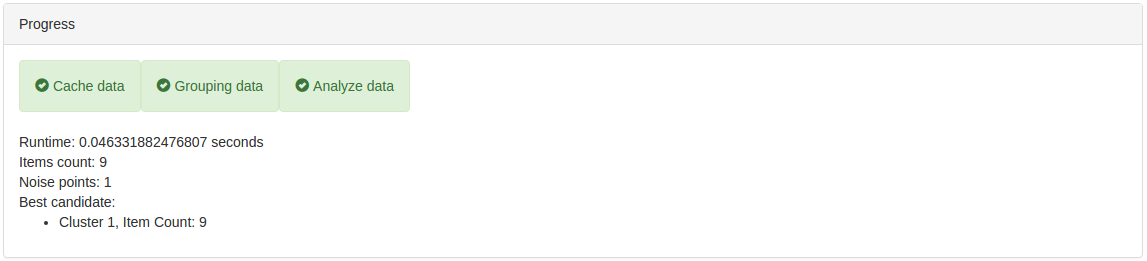
\includegraphics[width=1\textwidth]{images/tc11-dbscan-1}
		\caption{Generelle Informationen}
		\label{fig:testingfazit:testing:testcases:11-1-1}
	\end{subfigure} \\
	\begin{subfigure}[t]{1\textwidth}
		\centering
		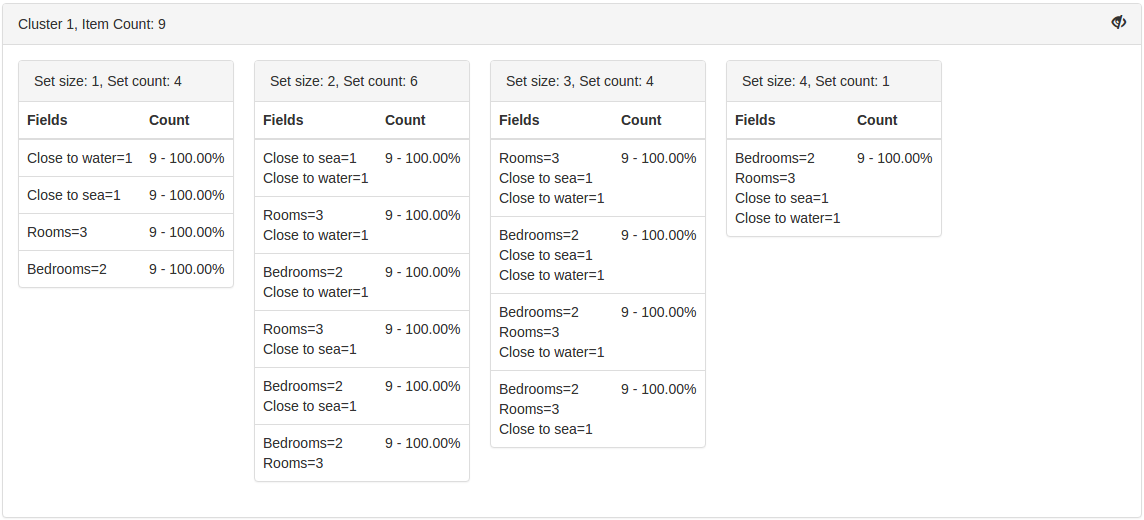
\includegraphics[width=1\textwidth]{images/tc11-dbscan-2}
		\caption{Cluster 1}
		\label{fig:testingfazit:testing:testcases:11-1-2}
	\end{subfigure}
	\caption{TC11 - Ausgabe des Programmes - Resultat des DBSCAN Algorithmus}
	\label{fig:testingfazit:testing:testcases:11-1}
\end{figure}

\begin{longtable}{ | l | l | l | l |} 	
	\hline 
	\rowcolor{tableheadcolor}
	\multicolumn{4}{|l|}{\bfseries ID: TC11-2 k-prototype} \\ \hline 
	Datebquelle & \multicolumn{3}{|l|}{\cref{app:testdatenquellen:11}} \\ \hline 
	Dateneinschränkung & \multicolumn{3}{|l|}{Keine} \\ \hline 
	
	\rowcolor{tableheadcolor}
	\multicolumn{4}{|l|}{\bfseries Erwartetes Resultat} \\ \hline 
	
	\multicolumn{4}{|l|}{\textbf{Cluster 1}} \\ \cline{2-4} 
	& Fehler & \multicolumn{2}{|l|}{0} \\ \cline{2-4} 
	& Grösse & \multicolumn{2}{|l|}{9} \\ \cline{2-4} 
	& \multicolumn{3}{|L{7.5cm}|}{Das Resultat der Analyse dieses Clusters vom Apriori Algorithmus ist dasselbe wie jenes vom DBSCAN welches oben aufgeführt wurde. Zur Verbesserung der Übersicht wird das Resultat hier nicht noch einmal aufgeführt.} \\ \hline
	
	\multicolumn{4}{|l|}{\textbf{Cluster 2}} \\ \cline{2-4} 
	& Fehler & \multicolumn{2}{|l|}{0} \\ \cline{2-4} 
	& Grösse & \multicolumn{2}{|l|}{1} \\ \cline{2-4} 
	& \multicolumn{3}{|L{7.5cm}|}{Der Apriori Algorithmus findet keine häufigen Attribute, da $minsup$ auf 0.2 (oder 20\%) gesetzt ist und nur 1 Element in diesem Cluster vorhanden ist.} \\ \hline
	
	
	\rowcolor{tableheadcolor}
	\multicolumn{4}{|l|}{\bfseries Tatsächliches Resultat} \\ \hline 
	
	\multicolumn{4}{|l|}{\textbf{Cluster 1}} \\ \cline{2-4} 
	& Fehler & \multicolumn{2}{|l|}{0} \\ \cline{2-4} 
	& Grösse & \multicolumn{2}{|l|}{9} \\ \cline{2-4} 
	& \multicolumn{3}{|L{7.5cm}|}{Das Resultat der Analyse dieses Clusters vom Apriori Algorithmus ist dasselbe wie jenes vom DBSCAN welches oben aufgeführt wurde. Zur Verbesserung der Übersicht wird das Resultat hier nicht noch einmal aufgeführt.} \\ \hline
	
	\multicolumn{4}{|l|}{\textbf{Cluster 2}} \\ \cline{2-4} 
	& Fehler & \multicolumn{2}{|l|}{0} \\ \cline{2-4} 
	& Grösse & \multicolumn{2}{|l|}{1} \\ \cline{2-4} 
	& \multicolumn{3}{|L{7.5cm}|}{Der Apriori Algorithmus findet keine häufigen Attribute, da $minsup$ auf 0.2 (oder 20\%) gesetzt ist und nur 1 Element in diesem Cluster vorhanden ist.} \\ \hline
	
	\rowcolor{tableheadcolor}
	\multicolumn{4}{|l|}{\bfseries Testergebnis} \\ \hline 
	\multicolumn{4}{|l|}{\cellcolor{green!25}} \\ \hline 
	
	\caption{TC11-2 Auswertung vom k-prototype Algorithmus}
	\centering
	\label{fig:testingfazit:testing:testcases:11:2}
\end{longtable}
\begin{figure}[H]
	\begin{subfigure}[t]{1\textwidth}
		\centering
		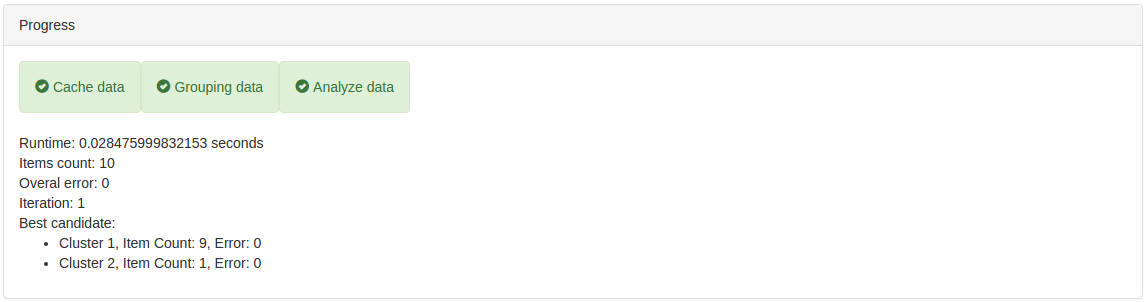
\includegraphics[width=1\textwidth]{images/tc11-kprototype-1}
		\caption{Generelle Informationen}
		\label{fig:testingfazit:testing:testcases:11-2-1}
	\end{subfigure} \\
	\begin{subfigure}[t]{1\textwidth}
		\centering
		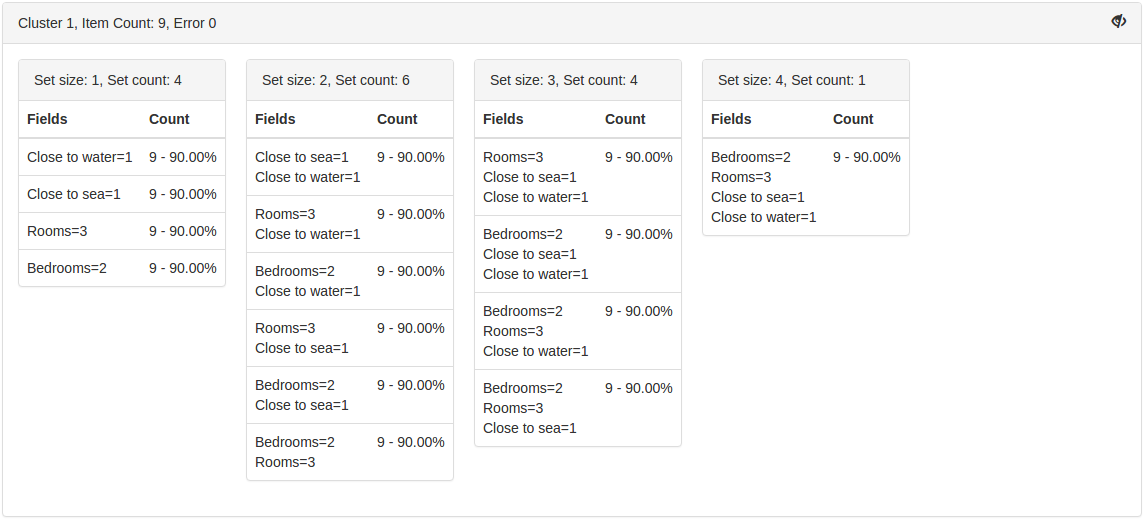
\includegraphics[width=1\textwidth]{images/tc11-kprototype-2}
		\caption{Cluster 1}
		\label{fig:testingfazit:testing:testcases:11-2-2}
	\end{subfigure}
	\begin{subfigure}[t]{1\textwidth}
		\centering
		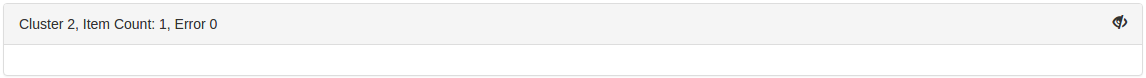
\includegraphics[width=1\textwidth]{images/tc11-kprototype-3}
		\caption{Cluster 2}
		\label{fig:testingfazit:testing:testcases:11-2-3}
	\end{subfigure}
	\caption{TC11-2 - Ausgabe des Programmes - Resultat des k-prototype Algorithmus}
	\label{fig:testingfazit:testing:testcases:11-2}
\end{figure}

\begin{longtable}{ | l | l | l | l |} 	
	\hline 
	\rowcolor{tableheadcolor}
	\multicolumn{4}{|l|}{\bfseries ID: TC12-1 DBSCAN} \\ \hline 
	Datebquelle & \multicolumn{3}{|l|}{\cref{app:testdatenquellen:12}} \\ \hline 
	Dateneinschränkung & \multicolumn{3}{|l|}{Keine} \\ \hline 
	
	\rowcolor{tableheadcolor}
	\multicolumn{4}{|l|}{\bfseries Erwartetes Resultat} \\ \hline 
	Noise Punkte & \multicolumn{3}{|l|}{1} \\ \hline 
	
	% ----------------------------------------------		
	\multicolumn{4}{|l|}{\textbf{Cluster 1}} \\ \cline{2-4} 
	& Grösse & \multicolumn{2}{|l|}{4} \\ \cline{2-4} 
	&& Attributmenge & Anzahl \\ \cline{2-4} 
	
	& 1er-Attributmenge & \tabitem Nahe am Meer & 4 \\ \hline
		
	% ----------------------------------------------		
	\multicolumn{4}{|l|}{\textbf{Cluster 1}} \\ \cline{2-4} 
	& Grösse & \multicolumn{2}{|l|}{5} \\ \cline{2-4} 
	&& Attributmenge & Anzahl \\ \cline{2-4} 
	
	& 1er-Attributmenge & \tabitem Aircondition & 4 \\ \cline{3-4} 
	& & \tabitem Wochenpreis=günstig & 3 \\ \cline{3-4} 
	& & \tabitem Anzahl Zimmer=9 & 3 \\ \cline{3-4} 
	& & \tabitem Anzahl Schlafzimmer=8 & 3 \\ \cline{2-4} 
	
	& 2er-Attributmenge & \tabitem Anzahl Zimmer=9 & 3 \\
	& & \tabitem Wochenpreis=günstig & \\ \hline
		
		
	\rowcolor{tableheadcolor}
	\multicolumn{4}{|l|}{\bfseries Tatsächliches Resultat} \\ \hline 
		
	% ----------------------------------------------		
	\multicolumn{4}{|l|}{\textbf{Cluster 1}} \\ \cline{2-4} 
	& Grösse & \multicolumn{2}{|l|}{4} \\ \cline{2-4} 
	&& Attributmenge & Anzahl \\ \cline{2-4} 
	
	& 1er-Attributmenge & \tabitem Nahe am Meer & 4 \\ \hline
		
	% ----------------------------------------------		
	\multicolumn{4}{|l|}{\textbf{Cluster 1}} \\ \cline{2-4} 
	& Grösse & \multicolumn{2}{|l|}{5} \\ \cline{2-4} 
	&& Attributmenge & Anzahl \\ \cline{2-4} 
	
	& 1er-Attributmenge & \tabitem Aircondition & 4 \\ \cline{3-4} 
	& & \tabitem Wochenpreis=günstig & 3 \\ \cline{3-4} 
	& & \tabitem Anzahl Zimmer=9 & 3 \\ \cline{3-4} 
	& & \tabitem Anzahl Schlafzimmer=8 & 3 \\ \cline{2-4} 
	
	& 2er-Attributmenge & \tabitem Anzahl Zimmer=9 & 3 \\
	& & \tabitem Wochenpreis=günstig & \\ \hline

	\caption{TC12-1 Auswertung vom DBSCAN Algorithmus}
	\centering
	\label{fig:testingfazit:testing:testcases:12:1}
\end{longtable}
\begin{figure}[H]
	\begin{subfigure}[t]{1\textwidth}
		\centering
		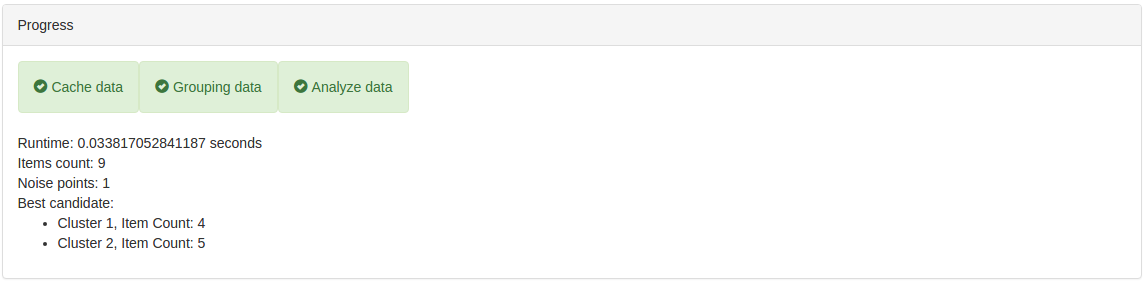
\includegraphics[width=1\textwidth]{images/tc12-dbscan-1}
		\caption{Generelle Informationen}
		\label{fig:testingfazit:testing:testcases:12-1-1}
	\end{subfigure} \\
	\begin{subfigure}[t]{1\textwidth}
		\centering
		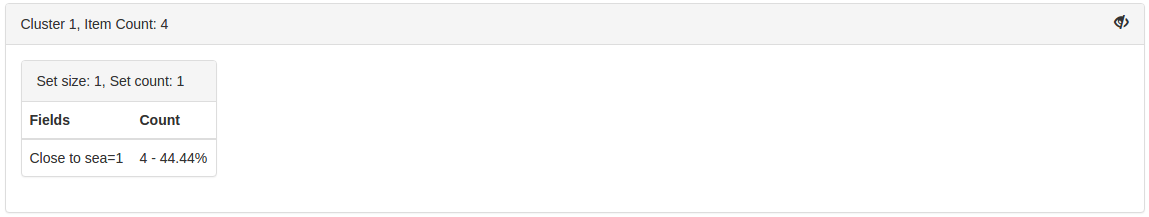
\includegraphics[width=1\textwidth]{images/tc12-dbscan-2}
		\caption{Cluster 1}
		\label{fig:testingfazit:testing:testcases:12-1-2}
	\end{subfigure}\\
	\begin{subfigure}[t]{1\textwidth}
		\centering
		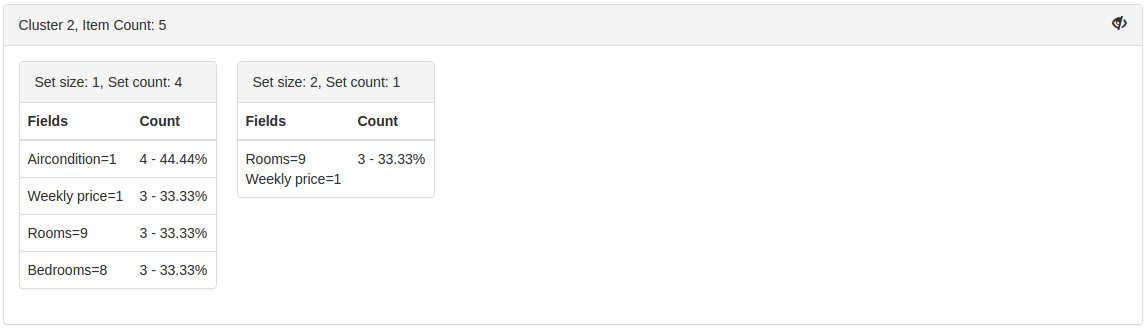
\includegraphics[width=1\textwidth]{images/tc12-dbscan-3}
		\caption{Cluster 2}
		\label{fig:testingfazit:testing:testcases:12-1-3}
	\end{subfigure}
	\caption{TC12 - Ausgabe des Programmes - Resultat des DBSCAN Algorithmus}
	\label{fig:testingfazit:testing:testcases:12-1}
\end{figure}

\begin{longtable}{ | l | l | l | l |} 	
	\hline 
	\rowcolor{tableheadcolor}
	\multicolumn{4}{|l|}{\bfseries ID: TC12-2 k-prototype} \\ \hline 
	Datebquelle & \multicolumn{3}{|l|}{\cref{app:testdatenquellen:12}} \\ \hline 
	Dateneinschränkung & \multicolumn{3}{|l|}{Keine} \\ \hline 
	
	\rowcolor{tableheadcolor}
	\multicolumn{4}{|l|}{\bfseries Erwartetes Resultat} \\ \hline 
		
	% ----------------------------------------------		
	\multicolumn{4}{|l|}{\textbf{Cluster 1}} \\ \cline{2-4}
	& Fehler & \multicolumn{2}{|l|}{6.086575} \\ \cline{2-4}  
	& Grösse & \multicolumn{2}{|l|}{5} \\ \cline{2-4} 
	&& Attributmenge & Anzahl \\ \cline{2-4} 
	
	& 1er-Attributmenge & \tabitem Nahe am Meer & 4 \\ \cline{2-4}
	& & \tabitem Nahe am ÖV (öffentlicher Verkehr) & 3 \\ \hline
		
	% ----------------------------------------------		
	\multicolumn{4}{|l|}{\textbf{Cluster 1}} \\ \cline{2-4} 
	& Fehler & \multicolumn{2}{|l|}{3.090957} \\ \cline{2-4} 
	& Grösse & \multicolumn{2}{|l|}{5} \\ \cline{2-4} 
	&& Attributmenge & Anzahl \\ \cline{2-4} 
	
	& 1er-Attributmenge & \tabitem Aircondition & 4 \\ \cline{3-4} 
	& & \tabitem Wochenpreis=günstig & 3 \\ \cline{3-4} 
	& & \tabitem Anzahl Zimmer=9 & 3 \\ \cline{3-4} 
	& & \tabitem Anzahl Schlafzimmer=8 & 3 \\ \cline{2-4} 
	
	& 2er-Attributmenge & \tabitem Anzahl Zimmer=9 & 3 \\
	& & \tabitem Wochenpreis=günstig & \\ \hline
		
		
	\rowcolor{tableheadcolor}
	\multicolumn{4}{|l|}{\bfseries Tatsächliches Resultat} \\ \hline 
			
	% ----------------------------------------------		
	\multicolumn{4}{|l|}{\textbf{Cluster 1}} \\ \cline{2-4}
	& Fehler & \multicolumn{2}{|l|}{6.086575} \\ \cline{2-4}  
	& Grösse & \multicolumn{2}{|l|}{5} \\ \cline{2-4} 
	&& Attributmenge & Anzahl \\ \cline{2-4} 
	
	& 1er-Attributmenge & \tabitem Nahe am Meer & 4 \\ \cline{2-4}
	& & \tabitem Nahe am ÖV (öffentlicher Verkehr) & 3 \\ \hline
		
	% ----------------------------------------------		
	\multicolumn{4}{|l|}{\textbf{Cluster 1}} \\ \cline{2-4} 
	& Fehler & \multicolumn{2}{|l|}{3.090957} \\ \cline{2-4} 
	& Grösse & \multicolumn{2}{|l|}{5} \\ \cline{2-4} 
	&& Attributmenge & Anzahl \\ \cline{2-4} 
	
	& 1er-Attributmenge & \tabitem Aircondition & 4 \\ \cline{3-4} 
	& & \tabitem Wochenpreis=günstig & 3 \\ \cline{3-4} 
	& & \tabitem Anzahl Zimmer=9 & 3 \\ \cline{3-4} 
	& & \tabitem Anzahl Schlafzimmer=8 & 3 \\ \cline{2-4} 
	
	& 2er-Attributmenge & \tabitem Anzahl Zimmer=9 & 3 \\
	& & \tabitem Wochenpreis=günstig & \\ \hline
		
	\caption{TC12-2 Auswertung vom k-prototype Algorithmus}
	\centering
	\label{fig:testingfazit:testing:testcases:12:2}
\end{longtable}
\begin{figure}[H]
	\begin{subfigure}[t]{1\textwidth}
		\centering
		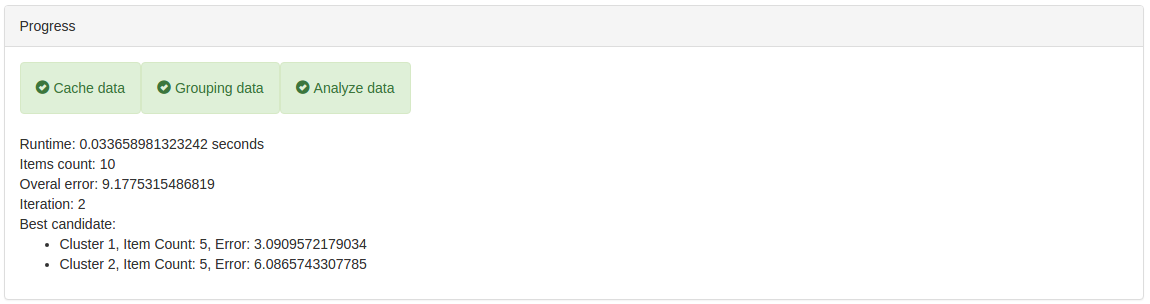
\includegraphics[width=1\textwidth]{images/tc12-kprototype-1}
		\caption{Generelle Informationen}
		\label{fig:testingfazit:testing:testcases:12-2-1}
	\end{subfigure} \\
	\begin{subfigure}[t]{1\textwidth}
		\centering
		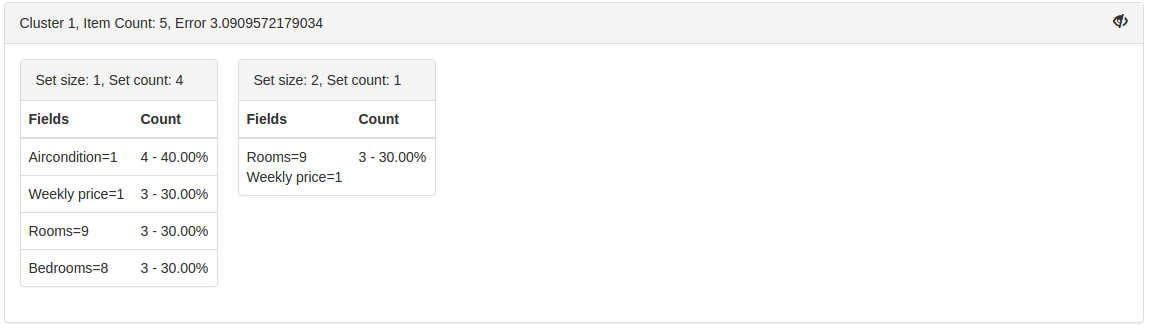
\includegraphics[width=1\textwidth]{images/tc12-kprototype-2}
		\caption{Cluster 1}
		\label{fig:testingfazit:testing:testcases:12-2-2}
	\end{subfigure}
	\begin{subfigure}[t]{1\textwidth}
		\centering
		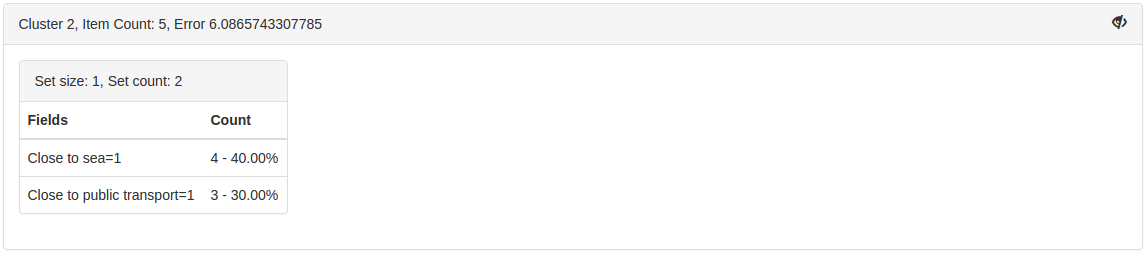
\includegraphics[width=1\textwidth]{images/tc12-kprototype-3}
		\caption{Cluster 2}
		\label{fig:testingfazit:testing:testcases:12-2-3}
	\end{subfigure}
	\caption{TC12-2 - Ausgabe des Programmes - Resultat des k-prototype Algorithmus}
	\label{fig:testingfazit:testing:testcases:12-2}
\end{figure}

\subsection{Hypothesen}
\label{sec:testingfazit:testing:hypothesen}
Im \cref{sec:einleitung:ziel:hypothesen} \nameref{sec:einleitung:ziel:hypothesen} sind Hypothesen aufgestellt worden welche auf ihre Richtigkeit geprüft wurden. Nachfolgend wird das Resultat vorgestellt.

%"`"'
\paragraph{Hypothese 1: "`Die meisten Kunden von Interhome kommen aus der Schweiz oder Frankreich"'} Durch eine Einschränkung der analysierten Attribute des Apriori Algorithmus auf das Herkunftsland des Kunden wurde diese Hypothese bestätigt. 20.94\% aller Buchungen wurden von Schweizer getätigt und 18.58\% von Franzosen. 
\paragraph{Hypothese 2: "`Die meisten Buchungen werden für die Schweiz und für Frankreich getätigt"'} Das Resultat des Apriori Algorithmus wurde für die Auswertung dieser Hypothese eingeschränkt, so dass nur der Standort des Objektes analysiert wird. Als Filter wurde gesetzt dass die Buchung aus der Schweiz stammen muss. Dadurch konnte die Hypothese bestätigt werden. 19.92\% aller Buchungen wurde für Objekte in der Schweiz getätigt, und 13.97\% für deren aus Frankreich.
\paragraph{Hypothese 3: "`Schweizer Kunden buchen meistens Objekte in der Schweiz."'} Eingeschränkt wurden die Attribute hier auf den Standort des Objektes. Zusätzlich wurde ein Filter gesetzt auf die Herkunft des Kunden. Als Resultat gab das Programm aus, dass 49.24\% aller Schweizer ein Objekt in der Schweiz buchen. Abgeschlagen auf dem zweiten Platz rangiert Frankreich mit 7.34\% und danach Italien mit 6.99\%. Es ist generell gültig, dass meistens ein Ferienhaus im eigenen Land gebucht wird. Jedoch ist es nirgends so extrem wie in der Schweiz. Franzosen buchen mit 32.20\% am meisten Objekte in Frankreich und mit 16.50\% in Spanien. Italiener buchen zu 18.01\% Objekte in Italien und 17.11\% in Spanien.
\paragraph{Hypothese 4: "`Destinationen mit Meer Anschluss werden öfters Objekte mit mehreren Schlafzimmern gebucht"'} 
\paragraph{Hypothese 5: "`Schweizer Buchungen in Skiregionen sind nahe am Skilift oder am öffentlichem Verkehr"'} 
\paragraph{Hypothese 6: "`Zu kalten Jahreszeiten wird von Schweizern mehr Regionen am Meer gebucht als im Sommer."'} 
\paragraph{Hypothese 7: "`Anfang des Jahres werden teurere Objekte gebucht als im Oktober, da der dreizente Monatslohn eingetroffen ist."'} 


\section{Fazit}

\section{Mögliche Erweiterungen/Verbesserungen}
Diskretiesierungsschritte \cref{sec:recherche:datenvorbereitung} nach Häufigkeitsanalyse.
Z.b. die Preise plotten -> man sieht ein peek bei CHF1000/Buchung. +/- 1/3 vom Peek sind die normalen Preise. Darunter Budget, darüber Luxury

\gls{optics} einsetzen um $\epsilon$ bei \gls{dbscan} zu eliminieren.

Hierarchical clustering einsetzen. Allerdings weniger performant und deshalb schlecht fürs explorieren geeignet.

Sockets einsetzen um Polling vom Webbrowser zu vermeiden.